%!TEX root = ../thesis.tex

\chapter{A Modular Software Framework for Autonomous Vehicles}
\label{ch:modular}

\ifpdf
	\graphicspath{{Chapter6/Figs/Raster/}{Chapter6/Figs/PDF/}{Chapter6/Figs/}}
\else
	\graphicspath{{Chapter6/Figs/Vector/}{Chapter6/Figs/}}
\fi

Software frameworks for autonomous vehicles are required to interface and process data from several different sensors on board the vehicle, in addition to performing navigational processes such as path planning and lane keeping. These can include a combination of cameras, LiDARs, GPS, IMU, and odometric sensors to achieve positioning and localisation for the vehicle and can be challenging to integrate. In this paper, we present a unified software framework that combines sensor and navigational processing for autonomous driving. Our framework is modular and scalable whereby the use of protocol buffers enables segregating each sensor and navigation subroutine individual classes, which can then be independently modified or tested. It is redesigned to replace the existing software on our Formula SAE vehicle, which we use for testing autonomous driving. Our testing results verify the suitability of our framework to be used for fully autonomous drives.

\section{Introduction}
UWA's Renewable Energy Vehicle Project (REV) operates two autonomous vehicles, a BMW X5 and a student-built Formula SAE-Electric car. Formula SAE~\cite{sae_international_student_nodate} is a long-running annual competition organised by the Society of Automotive Engineers with competition events worldwide. The design competition includes petrol cars, as well as the SAE-Electric class which includes ours with two electric motors driving each of the two rear wheels via independent controllers. We have incorporated full drive-by-wire control of the throttle, steering and the hydraulic braking system. The use of a Formula SAE car provides several advantages for such a project; the car is mechanically simple, Formula SAE cars with similar designs are common at universities worldwide and the size of the car makes testing accessible without forgoing race car vehicle dynamics. Furthermore, the use of an electric vehicle makes the project significantly more practical for student work as the risks and environmental issues associated with petrol-engine cars are eliminated and the systems installed in this project can take advantage of the large amount of electrical energy already available on the vehicle.

For the driverless FSAE project, our goal was to be able to autonomously drive a vehicle around a race track. This is being achieved by placing waypoints along the ideal driving line, as well as ``fence points" to lock out non-driving areas. Maps can either be recorded by human or remote-controlled driving or specified through a Google Maps driven web-interface. During autonomous driving, a laser scanner and camera are used for detection of road edges as well as any obstacles on the track. Safety systems are essential for a driverless system, as the car weighs more than 250 kg and is capable of driving at a speed of 80 km/h. Both the low-level drive-by-wire, as well as high-level navigation system have independent safety systems built in. These include remote intervention, remote heartbeat and remote emergency stopping, which are implemented through a fail-safe wireless link to a base station as well as through hard-wired buttons on the car itself. 

\nomenclature[z-fsae]{FSAE}{Formula SAE}

Our motivation for designing and presenting this framework is to improve upon the existing autonomous drive software on our SAE vehicle that is documented in~\cite{drage_development_2013}. This software utilises a web-based user interface (UI) that displays via a touch screen mounted in the vehicle’s cockpit. Our proposed framework utilises this existing UI with a revamped backend as described in Section~\ref{sec:6:autonomous}. It was noted that the existing software had a heavy reliance on a central Control module, which required all the sensors and their submodules to run to function. These submodules were programmed throughout the years with different programming languages and redundancies, which made integration difficult. Our proposed framework presents a streamlined approach whereby each module will be programmed with a C++ interface that communicates with either a path planner or a drive control system. This system also benefits from additional features including visualisation data playback (online or offline) and a web-based user interface. As a customised framework for our project, this also alleviates the reliance on node-based solutions such as ROS, which usually requires a perpetually running Master node to function and allows higher reliability when the individual components are integrated.

\nomenclature[z-ui]{UI}{User interface}

Additionally, this approach presents a long-term advantage whereby our framework is made fully open and contributable by students and enthusiasts looking to implement our framework onto their custom-fabricated vehicles. When compared against other autonomous driving frameworks such as Apollo~\cite{baidu_apollo_nodate} and Autoware~\cite{autoware_autoware_nodate} that mostly target commercial vehicles and requiring expensive hardware, our approach leverages on hardware and fabrication methods that are more accessible in cost.

\section{Autonomous Driving Framework}\label{sec:6:autonomous}
\begin{sidewaysfigure}
	\centering
	\includegraphics[width=\linewidth] {arch}
	\caption{The software architecture diagram of our proposed framework.}
	\label{fig:6:arch}
\end{sidewaysfigure}

This section introduces our proposed software framework for the SAE vehicle, with the software architecture diagram as illustrated in Fig.~\ref{fig:6:arch}. The software architecture of the vehicle utilises a modular design to allow for continuous parallel development on each of the sensors, the path planning algorithm, and the control policy. Input sensors are comprised of the LiDAR, camera, GPS, IMU and four wheel speed sensors, which are required to function simultaneously in order for the car to drive autonomously. The LiDAR, camera, GPS and IMU each have their own receiver class on the Jetson TX1, which takes the input from the sensors and processes the data. Additionally, rotary-encoder odometry is performed using an Arduino microcontroller connected to each of the wheels' encoder. This information is received in the high-level software by another receiver class which processes the data to produce wheel speed measurements. Relevant data for path planning and localisation is encoded in protobuf~\cite{google_developers_protocol_nodate} format and then passed to either the path-planning program or the control program, which performs localisation as well as some communication and logging utilities. The control program also communicates with the web GUI, providing a visualisation of the data and allows the user to start and stop autonomous driving as well as the safety trip monitor and the controller, thereby introducing a high-level interface for driving the car. The control program, once it has communicated with the path-planner to combine localisation data with a set of future way points, will transmit driving instructions to the controller. This in turn transmits them to a low-level microcontroller. Not pictured in the diagram is the fusion of data from sources such as the GPS and IMU, and IMU and LiDAR in order to improve the accuracy of localisation. Detailed explanations of the sensors and classes are covered in Sections~\ref{sec:6:pathplanner} through~\ref{sec:6:controller}.

\subsection{Path Planner}\label{sec:6:pathplanner}
We use a real-time capable path-planning algorithm based on~\cite{chu_local_2012}.
Given a set of pre-recorded or pre-defined waypoints along a track, the planner will generate a optimised path through all way points, which serves as a base frame for trajectory generation.
During operation, the algorithm evaluates a variety of possible trajectories in the configurations space of the vehicle using rapidly-exploring random trees (RRTs)~\cite{lavalle_planning_2006}.
Those intermediate trajectories are generated along a curvilinear coordinate system, along with the base frame.
Each possible trajectory is checked for collisions with obstacles. A collision free path is then picked, utilizing a cost-function, that enables us to influence the driving style of the vehicle.
The algorithms are implemented in C++14 and rely heavily on the C++ source libraries Boost and Eigen3.

\nomenclature[z-rrt]{RRT}{Rapidly-exploring random tree}

We use an arc-length parametrised cubic B-spline $P_b(s)$~\cite{wang_arc-length_2002} to generate a base frame for the curvilinear coordinate system, which can be described as a non-linear transformation of the parameter domain on the four waypoints $a$ to $d$, parametrised by $s$.
\begin{align}
	P_b(s) = \begin{cases}
	x_b(s) & = a_{x,i}(s - s_i)^3 + b_{x,i}(s - s_i)^2   + c_{x,i}(s - s_i) + d_{x,i} \\
	y_b(s) & = a_{y,i}(s - s_i)^3 + b_{y,i}(s - s_i)^2   + c_{y,i}(s - s_i) + d_{y,i} \\
	\end{cases}
\end{align}
The curvature $\kappa_b$ can be calculated from the first and second derivatives of $P_b(s)$
\begin{align}
\kappa_b = \frac{x'_by''_b - x''_by'_b}{(x'^2_b - y'^2_b)^\frac{3}{2}} &
\end{align}
where:
\begin{subequations}
	\begin{align}
	\frac{dx_b}{ds} &= x_b' = \cos\theta_b \\
	\frac{dy_b}{ds} &= y_b' = \sin\theta_b
	%\frac{d^2x_b}{ds^2} = x_b'' &\qquad \frac{d^2y_b}{ds^2} = y_b''\\
	\end{align}
\end{subequations}
The curvature of a cubic spine is continuous in all sections.
For this reason, a parametric cubic B-spline is adopted for the base frame.
Since the position of the vehicle is provided in Cartesian-space, we need to find a transform those coordinates to a curvilinear representation, of which the B-spline provides the base.
This is equal to finding the closest point to the vehicle on the base frame, by minimising the Euclidean distance between the position of the vehicle and the cubic B-spline.
\begin{equation}
\min_s d(s) = \sqrt{[x_v - x_b(s)]^2+[(y_v - y_b(s)]^2}
\end{equation}
We chose Brent's method~\cite{brent_algorithms_1973} to find the minimum. Another suitable and stable algorithm is provided in~\cite{xu_accurate_2008}.
From the lateral distance to the base frame and the base frame we construct the curvilinear coordinate system in which we generate a number $n$ of paths as cubic polynomials.
Each polynomial is defined by a lateral offset $q(s)$ and a curvature $\kappa$, to cover a broad section of the configuration space of the vehicle.
$n$ is a design parameter and can be chosen to adjust the computational load of the algorithms.
We now design a vehicle model of a set of differential equations in Cartesian space.
\begin{subequations}
	\begin{align}
	\dot{x} &= v \cos\theta \\
	\dot{y} &= v \sin\theta \\
	\dot{\theta} &= v\kappa
	\end{align}
\end{subequations}
This vehicle model is transformed onto the curvilinear coordinate system, and the position of the vehicle in Cartesian space can then be determined by forward integration.
Paths that violate the nonholonomic constraints of vehicle motions or collide with an obstacle are eliminated.
The remaining paths are evaluated by a construction. 
The cost function itself can be chosen to optimise driving for an arbitrary property, like sportiness or safety.
By simulating the path planner using equally weighted costs, the near-optimal path can be obtained as Fig.~\ref{fig:6:loop}, with the path drawn in green and the base frame in blue. The manoeuvre selection is subsequently presented as Fig.~\ref{fig:6:mano} 
Because this planner insoles a simple vehicle model as a set of ordinary differential equations, it can be conveniently integrated into any control algorithm.

\nomenclature[g-k]{$\kappa$}{Curvature}
\nomenclature[g-t]{$\theta$}{Angular orientation}
\nomenclature[a-s]{$s$}{Paramaterisation}   
\nomenclature[s-t]{$b$}{B-spline}   
\nomenclature[a-n]{$n$}{Integer set}   
\nomenclature[a-v]{$v$}{Velocity}   
\nomenclature[a-v]{$d$}{Euclidean distance}   

\begin{figure}[H]
	\centering
	\begin{subfigure}[b]{0.45\textwidth}
		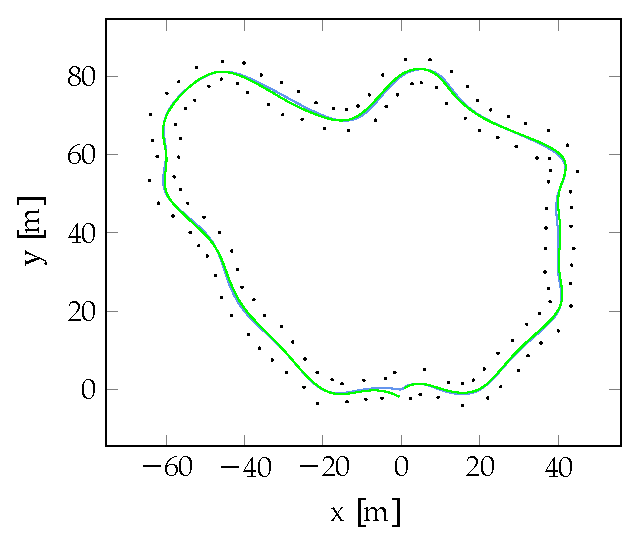
\includegraphics[width=\textwidth]{pathloop}
		\caption{Simulated path}
		\label{fig:6:loop}   
	\end{subfigure} 
	\hspace{1em}         
	\begin{subfigure}[b]{0.45\textwidth}
		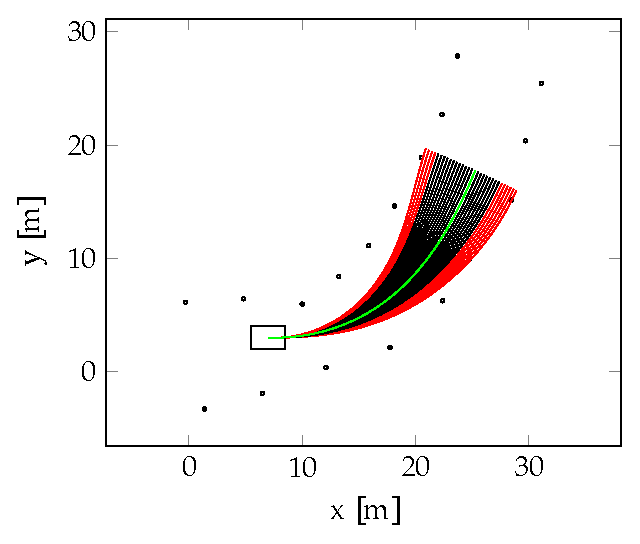
\includegraphics[width=\textwidth]{manoeuvre}
		\caption{Manoeuvre selection}
		\label{fig:6:mano}
	\end{subfigure}             
	\caption[Simulated near-optimal path and manoeuvre selection]{Simulated near-optimal path (a) and manoeuvre selection (b). Black dots represent road delimiters.}
	\label{fig:6:loopmano}
\end{figure}

\subsection{Software Communications}
The sensors on the vehicle communicate with the path planner using procotol buffers. Protocol Buffers (protobuf)~\cite{google_developers_protocol_nodate} are a formalised data structure developed by Google for use in cross-platform systems. Protobuf allows for the combination of several standard variables into a single packed structure that can be easily serialised and accessed using automatically generated methods. The protobuf library has bindings for many common programming languages, including C++, Python and Java, meaning that a protobuf structure packaged in a C++ application, can be read in by a Java application with no conversion needed. 

\nomenclature[z-protobuf]{Protobuf}{Protocol buffer}

Protocol buffers are used internally within our software as regularly structured state variables, with easy to use member functions. For example, the GPS software stores its current state within a protobuf object containing data such as latitude, longitude, ground speed and angle. This GPS state can then be used by internal code regularly, or it can be used serialised and stored.  The serialised protobuf data is very compact and space efficient, meaning that a huge amount of logged data can be saved sequentially. 

By abstracting the actual data from a specific sensor behind a protobuf object, it allows for the use of Polymorphism within our software, and so dependencies on a specific piece of hardware are loosened. As long as a specific hardware device can be interpreted into the appropriate protobuf form,  it can be integrated easily into the system, with only short wrapping code needed to be written. There is also no dependency for this protobuf data to come from a physical sensor, the protobuf data can be read in from a previously serialised log, allowing for the replay of data, or it can be read from an external piece of software, allowing for the use of simulation programs.

\subsection{Localisation}
The vehicle achieves localisation through the inertial measurement unit (IMU) and global positioning system (GPS). The IMU used in the project is the Xsens MTi~\cite{xsens_mti_nodate} 9 depth-of-field sensor. The sensor contains several advanced internal algorithms in order to provide accurate and noise-free measurements of the current gyroscopic position, the acceleration, and the magnetic field. These values are returned by the IMU readings as the velocity, acceleration, and the three rotations (pitch, roll and yaw) along the $x$, $y$ and $z$ axis. The sensor is used within the project to determine heading, and assist in the calculation of local positions. 

The GPS receiver used is the Columbus V-800 GPS receiver. It is used with the GPSd~\cite{raymond_gpsd_nodate} software to parse the National Marine Electronics Association (NMEA) standard data outputted by the GPS unit, and retransmit internally in an easier to use format. The data used from the GPS unit are the GPS coordinates, the ground speed, and the heading.  These GPS coordinates are first converted into a local reference frame, as a distance from a datum point. 
The acceleration and position data from the IMU and the GPS units respectively are fused together using an extended Kalman filter (EKF), producing a value for positioning that has a higher accuracy than GPS alone. This fusion system outputs the filtered position, velocity, and acceleration data which is then fed into the Path Planner and Control modules along with the bearing to ensure that the vehicle can reliably localise itself and obtain accurate readings for the position, velocity and acceleration. 

\nomenclature[z-nmea]{NMEA}{National Marine Electronics Association}

\subsection{Odometry}
The SAE car has been fitted with Hall Effect sensors that send its data through a comparator and an OR gate, this makes a pulse train where we use an Arduino UNO~\cite{arduino_arduino_nodate} to count the time between pulses to give angular velocity, which can be translated to meters per second. This gives the car Odometry, in which software will use an EKF to fuse the measurements together to improve their individual measurements and the vehicles’ localization capabilities. As the Arduino UNO is too slow to control the steering as well as breaking for the SAE Car, we added a second Arduino to do the odometry which then sends the data through serial communications to the main Arduino Nano. This low-level communicates steering and wheel velocity to the Nvidia Jetson TX1 for processing the data through the EKF, using a simple car kinematic model. The goal is to achieve the localization with reduced reliance on the GPS.

\subsection{LiDAR}
The Autonomous Formula SAE vehicle uses an ibeo LUX~\cite{autonomoustuff_ibeo_nodate} Light Distance and Ranging system (LiDAR) to sense distance information about the world around it. The LiDAR records the time interval between emission and recapture of thousands of infra-red light pulses to record a stream of 3-Dimensional points. The LiDAR is specifically designed for automotive purposes and is capable of internal data analysis; detecting and classifying objects in its field of vision. The LiDAR connects via an Ethernet switch to the Nvidia Jetson TX1~\cite{nvidia_corporation_embedded_2017-1}. A LiDAR reader class receives the serial bytestream which is continuously being transmitted. The data parsing is handled by the parser class which converts the bytestream into Protobuf objects. This format facilitates the storage and sharing of the information to the LiDAR visualisation.

\begin{figure}[H]
	\centering
	\includegraphics[width=0.8\linewidth]{luxplot}
	\caption[LiDAR plot at the position of Fig.~\ref{fig:6:carpark}]{LiDAR plot showing the detected parked vehicles at the position where Fig.~\ref{fig:6:carpark} was captured. The graph axes measure distances in metres.}
	\label{fig:6:lidar}
\end{figure}

Road-edge detection is achieved through the use of the LiDAR data. The LiDAR, aimed at an angle below horizontal beyond the front of the car, provides four layers of depth information with a horizontal angle of 85 degrees. Its output is visualised as Fig.~\ref{fig:6:lidar}. Road edge detection is achieved by analysing the depth information in one of the layers and checking it for both smoothness and slope. The central data points and those near them are considered and checked to confirm that they meet the slope criteria (the road should be relatively flat so no great changes in depth should be noted in a line) iteratively further and further points are considered in a stepwise process where the correlation coefficient is considered at each point. The road edge is the point at which the correlation coefficient is the highest whilst the slope condition is still being met. This approach was improved with the implementation of a Kalman filter which creates a time-averaged estimate of the road edge-position assisting in the prediction of the current road edge.

\subsection{Visual Navigation}\label{sec:6:visual}
The SAE vehicle uses visual information as one of its references for driving decisions. It mainly uses an off-the-shelf monocular camera to collect images then applied through OpenCV and SegNet~\cite{badrinarayanan_segnet:_2017} for road edges detection. OpenCV provides many modules, such as image processing, video, and video input/output, that is useful for road edges detection. However, using OpenCV alone for image recognition is limited by variations in image quality, brightness, and contrast. SegNet is an image semantic segmentation approach. It can classify road scene objects, such as the pedestrian, lane marking, traffic light, vehicles etc., that complement the insufficient of single image processing scheme. SegNet is a pixel-wise semantic segmentation in deep learning framework. Semantic segmentation is used to apply for understanding the visual scene and object. This has been widely adopted in autonomous driving. The architecture of SegNet is a convolution encoder and decoder which is a pixel-wise classifier. The objects classify from SegNet is including following classes, sky, Building, column-pole, road-marking, road, pavement, tree, sign-symbol, fence, vehicle, pedestrian, and bicyclist. The accuracy of classify result is 65.9\% for classes average~\cite{badrinarayanan_segnet:_2017}. The input images utilise SegNet to perform visual scene classification. This will produce results whereby road, road-marking, and pavement are classified (see Fig.~\ref{fig:6:carpark}), which is useful for road edges detection. OpenCV is simultaneously used to perform image processing. The first step for image processing is camera calibration to get an undistorted image. This is achieved using a chess board image and finding chess board corners to get two accumulated list --- 3D point in real world space and 2D points in an image plane. Then we use the camera calibration function in the OpenCV library to obtain the camera calibration and distortion coefficients. This scheme will remove camera distortions.

\begin{figure}[H]
	\centering
	\includegraphics[width=0.8\linewidth]{2}
	\caption{Segmentation results from a parking area on campus grounds.}
	\label{fig:6:carpark}
\end{figure}

The road edges detection scheme detects lane-marking at two sides of autonomous SAE vehicle. The lane-marking detection can also be performed solely by the OpenCV library. Finding the edges of the whole image will reduce the image complexity because numbers of colour and gradient of the image would make image processing more difficult. Canny edge detection~\cite{canny_computational_1986} is a convenient approach in found in the OpenCV library that can be applied for this purpose. Then, Hough transform~\cite{hough_method_1962} can be applied onto the image to detect the lanes on both sides of autonomous SAE vehicle. The marking of lanes is detected then using perspective transforms to get a bird’s eye view-like image. It can easily find the four points to represent the lane marking pair, where a second order polynomial method can be applied to fit the points. The lane distances are obtained using pixel values that are converted into metres. The scaling factors are according to the Australian road width standard of 3.3 to 3.5 metres. However, the image processing approach might fail because the lane markings are not clear or when there are no lane markings. Therefore, using SegNet's results can effectively circumvent this drawback due to its ability to robustly detect and classify road and lane markings, whereby the same road distance calculation can be applied to find the vehicle's distances to the road edges.

\subsection{Safety Trip Monitor}
The safety trip monitor was designed with an observer-notifier structure. Any of the objects responsible for performing a safety-crucial function in the software can call a trip on the trip state monitor. This includes the low-level safety software, the controller, the GPS software, the web interface, the heart beat and the car network. The trip state is stored by the trip state monitor and pushed to any object which implements the trip state observer class and has registered itself with the monitor. The observer class ensures that the trip state does not produce any irregular operations while driving. The observers which receive the trip state upon each change are attached to the monitor after its instantiation, which means that the set of objects in the software which can change the trip state and which need to track to trip state can be completely reconfigured without needing to make changes to the trip state monitor or observer classes. This is an ideal structure for the software of a research autonomous vehicle, as the continuous development of ongoing research will frequently modify the structure of functions of portions of the software while seeking to maintain the integrity of safety features, like the safety trip.

\subsection{Controller} \label{sec:6:controller}
The controller class is the high-level interface for the drive-by-wire functionality of the vehicle. The actual drive-by-wire controlling of the vehicle is done by separate software on an Arduino microcontroller. The controller class is the only high-level software which communicates with the low-level controller. The program utilizes three PID controllers to set the throttle, brake, and steering values. The controller class provides a high-level interface with methods to begin to stop autonomous control of the throttle, brake, and steering, as well as methods to set the bearing or speed of the vehicle with desired values. This interface is utilized by the Control program, which handles path planning, and the Fusion program, which provides fused IMU-GPS data in order to facilitate waypoint-based driving. Fig.~\ref{fig:6:base frame} and~\ref{fig:6:curvature} illustrates the base frame and curvature output by the path planner using the Control program based on our evaluation path in Section~\ref{sec:6:implement}. A large change in curvature is present where the U-turn was made.

\nomenclature[z-pid]{PID}{Proportional--integral--derivative (controller)}

\begin{figure}[H]
	\centering
	\begin{subfigure}[b]{0.45\textwidth}
		\def\svgwidth{\textwidth}
		\input{Chapter6/Figs/PDF/baseframe.pdf_tex}
		\caption{Baseframe trajectory}
		\label{fig:6:base frame}   
	\end{subfigure} 
	\hspace{1em}         
	\begin{subfigure}[b]{0.45\textwidth}
		\def\svgwidth{\textwidth}
		\input{Chapter6/Figs/PDF/curvature.pdf_tex}
		\caption{Derived curvature}
		\label{fig:6:curvature}
	\end{subfigure}             
	\caption[Generated trajectory base frame]{The trajectory base frame generated by the path planner (a) and its derived curvature (b).}
	\label{fig:6:basecurve}
\end{figure}

\section{Implementation on SAE Vehicle} \label{sec:6:implement}
The software for the autonomous driving system is programmed onto an Nvidia Jetson TX1  embedded computer that is mounted on the chassis of the vehicle. The environmental sensors namely the LiDAR, GPS, IMU and camera connects directly to the camera via Ethernet (LiDAR) and USB 2.0 (GPS, IMU, camera) respectively. This software can be implemented onto another vehicle so long as the same sensors are used, as the system outputs drive commands through the Control module, which can be configured according to the vehicle's hardware specifications. To test our system, we collected driving data with the vehicle driving in a parking area at the University of Western Australia (shown in Fig.~\ref{fig:6:map}) by recording readings from the GPU, IMU, LiDAR and camera. The GPS and IMU plots waypoints for the car, LiDAR performs obstacle detection, and the camera performs semantic segmentation. The test drive begins from the southern end and then driving towards the northern end before making a U-turn back to the vehicle's station position. The recorded waypoints are passed to the path planner, which generates a trajectory base frame as shown in Fig.~\ref{fig:6:base frame}. Subsequently, the curvature is obtained from the derivative of the base frame as Fig.~\ref{fig:6:curvature}, which can then be used to determine the steering angle for autonomous driving. 

\begin{figure}[H]
	\centering
	\def\svgwidth{0.7\linewidth}
	\input{Chapter6/Figs/PDF/map.pdf_tex}
	\caption{Map showing the path taken by the vehicle in with a solid red line.}
	\label{fig:6:map}
\end{figure}

\section{Results}
Fig.~\ref{fig:6:carpark} was captured while the car was driving northward as it approaches the end of its path. The input image is displayed on the left and its semantic segmentation result is displayed on the right image. Results from semantic segmentation showed that the road is properly classified, along other elements in the frame. Its LiDAR readings at that position is as illustrated in Fig.~\ref{fig:6:lidar}, whereby the parked vehicles are detected on the left, along with the vegetation in the distance and the wall on the right side of the vehicle. The combination of LiDAR and semantic segmentation enables the vehicle to understand its position on the road, along with the obstacle types and the distances to each obstacle. For further results on road and lane marker detection, we processed a drive recording from Udacity's Self-Driving Car Nanodegree~\cite{udacity_self-driving_2017}. From Fig.~\ref{fig:6:segnetroad}, the input image (Origin) is used for both semantic segmentation (SegNet), and bird's eye view transformation (Bird view). The system was able to identify objects on the road scene, and the curvature of the road can be calculated using the bird's eye view. The distance between the centre of the vehicle and the left and right lane markers are calculated as shown in the output. This is accompanied with a confidence value whereby a successful detection of the road lane markings will be denoted with a ``1''.  

\begin{figure}[H]
	\centering
	\includegraphics[width=0.8\linewidth]{segnet_road}
	\caption[Visual navigation output]{Original and Jetson TX1 output showing segmentation, bird’s eye view, vehicle distance to left and right lane marks.}
	\label{fig:6:segnetroad}
\end{figure}

\section{Conclusion}
In this paper, we have designed and demonstrated the functionality of our software framework that is implemented on our autonomous SAE vehicle. This framework is designed to cohesively interface with the vehicle's camera, LiDAR, GPS, IMU and wheel speed sensors while being capable of performing navigational tasks such as path planning, image processing, odometry, localisation, safety checks, speed and steering control. Each sensor and navigation task is programmed as a separate module to ensure modularity and scalability, allowing for each module to be changed independently. Protocol buffers handle intermodular communications, whereby each process parses its output as a protobuf to be sent to another module. With this framework implemented on the Jetson TX1, our test drives on the autonomous SAE vehicle was able to achieve results that are adequate for fully autonomous driving. Future works will include further testing of the autonomous navigation software and refinements to the control and path planner classes to ensure that the system is capable for road drives using full automation. 